\documentclass[conference]{IEEEtran}
\IEEEoverridecommandlockouts

\usepackage{cite}
\usepackage{amsmath,amssymb,amsfonts}
\usepackage{graphicx}
\usepackage{textcomp}
\usepackage{xcolor}
\usepackage{booktabs}
\usepackage{multirow}
\usepackage[caption=false,font=footnotesize]{subfig}
\usepackage{url}

\graphicspath{{assets/}}

\def\BibTeX{{\rm B\kern-.05em{\sc i\kern-.025em b}\kern-.08em
    T\kern-.1667em\lower.7ex\hbox{E}\kern-.125emX}}

\begin{document}

\title{TSC-Fusion: Thermohaline-Structured Spectral and 3D Ensemble Learning for Ocean Temperature and Salinity Prediction}

\author{
\IEEEauthorblockN{Shengxiang Yang\textsuperscript{1},
Zhibo Zhou\textsuperscript{1},
Xiaoyi Zhang\textsuperscript{1},
Yuchen Liu\textsuperscript{1}, and
Shiming Lin\textsuperscript{1,2,3}}
\IEEEauthorblockA{\textsuperscript{1}School of Informatics, Xiamen University, Xiamen, China}
\IEEEauthorblockA{\textsuperscript{2}School of Information Engineering, Changji University, Changji, China}
\IEEEauthorblockA{\textsuperscript{3}Key Laboratory of Southeast Coast Marine Information Intelligent Perception and Application, MNR, Zhangzhou, China\\
Corresponding author: xmulsm@xmu.edu.cn}
}

\maketitle

\begin{abstract}
Accurate three-dimensional temperature and salinity prediction from multi-source ocean observations is essential for understanding subsurface thermal and haline dynamics, yet it remains challenging due to coupled physical signals that operate at distinct spatial and temporal scales. This paper presents TSC-Fusion, a thermohaline-structured fusion network that integrates four complementary modeling branches: a thermohaline structure coordinate (TSC) memory that routes water-column profiles through learned water-mass prototypes, a global spectral low-mode mixer that captures basin-scale teleconnections via Fourier-domain learning, a 3D spatiotemporal structure branch that preserves vertical coherence, and a gated ensemble head that stabilizes multi-step forecasts through spatially adaptive member weighting. The model is evaluated on a 20-epoch evaluation protocol in the Western Pacific against FuXi-Ocean, FuXi-ONS, and AxiomOcean reimplementations. TSC-Fusion achieves first-place results on both variables: temperature RMSE 0.1013\,$^\circ$C (MAE 0.0687, $R^2$ 0.9898) and salinity RMSE 0.3689 PSU (MAE 0.2317, $R^2$ 0.8795). Ablation experiments analyze the relative effects of each component, and TEOS-10-derived physical diagnostics confirm that the predicted fields preserve meaningful temperature-salinity coupling.
\end{abstract}

\begin{IEEEkeywords}
Ocean prediction, temperature and salinity, thermohaline structure, spectral learning, 3D spatiotemporal modeling, ensemble fusion.
\end{IEEEkeywords}

\section{Introduction}

Ocean temperature and salinity fields encode the physical state of the upper ocean and directly affect acoustic propagation, fishery resources, ecosystem response, and climate regulation~\cite{LiuYuLiangSanWeiHaiYangWenYanChangZhiNengYuBaoJiYingYongYanJiu2025,WangZhaoYingJiYuGaiJinBPNNDeShengSuChangFenCengJianMo2024,TangAnJiYuShenDuXueXiLianHeWOA18WenYanMoXingGouJianShengSuChang2024,DongZhiGuoHaiYangNuanHuaBeiJingXiaHaiYangYuYeZiYuanJiQiShengWuXiangYingDeYanJiuJinZhan2024,YangNingShengWoGuoHaiYangXinXingChanYeZhanLueGaiGuan2014,CuiWeiJiYuZaiFenXiShuJuDeQuanQiuHaiYangShuiTiHeReYanShuYunJiQiJiJieBianHua2023}. In practice, these fields must be inferred from heterogeneous observations: sparse in-situ profiles, remotely sensed surface states, and atmospheric forcing. This paper studies this setting as a spatiotemporal prediction problem: given historical multi-source ocean states, predict future three-dimensional temperature and salinity fields.

The core difficulty is that temperature and salinity are shaped by distinct physical processes operating at different scales. Temperature is strongly controlled by latitude, stratification, and seasonal heating, producing smooth large-scale gradients. Salinity is more localized---affected by precipitation, runoff, ocean circulation, and water-mass mixing---and often exhibits sharp fronts and subsurface extrema. Surface height anomalies and wind fields provide dynamic context, but they are observed on different grids and carry different noise characteristics. A useful prediction method must therefore solve three linked problems: joint modeling of multiple physical variables, recognition of multi-scale spatial-temporal phenomena, and robust generalization to unseen periods.

Traditional numerical ocean models such as HYCOM and ROMS represent circulation through physically grounded equations and coordinate systems~\cite{bleckOceanicGeneralCirculation2002,LiZhenXiTaiPingYangYangLiuXiTongDuiHaiPingMianGaoDuBianHuaDeXiangYingJiYuQuYuHaiYangMoShiROMSShiYan2025}. They provide physical consistency but are computationally expensive and depend on forcing, parameterization, and data assimilation choices. Deep learning offers a complementary route by learning nonlinear dependencies from large observational archives~\cite{zhaoDeepLearningOcean2024,boninoMachineLearningMethods2024}. Recent advances include global AI forecasting models that operate on spectral representations~\cite{bi2023accurate}, 3D spatiotemporal architectures for volumetric ocean prediction, and ensemble methods that combine multiple forecast members for stability. However, existing work tends to emphasize one aspect---global spectral modeling, 3D convolutions, or ensembling---in isolation. The ocean forecasting problem calls for an architecture that jointly addresses water-mass-aware representation, large-scale spectral teleconnection, 3D vertical structure preservation, and ensemble stabilization.

We propose TSC-Fusion, a thermohaline-structured fusion network that integrates four complementary modeling branches. The thermohaline structure coordinate (TSC) memory module explicitly encodes water-mass information by soft-routing each water-column profile to learned prototypes, capturing the temperature-salinity-density-spiciness relationships that define distinct water masses. The global spectral low-mode branch learns basin-scale teleconnections by operating in the Fourier domain, modeling the low-frequency modes that govern large-scale gradients. The 3D spatiotemporal structure branch preserves vertical coherence through 3D convolutions over the joint variable-time-latitude-longitude cube. A gated ensemble head produces multiple forecast members and fuses them through spatially adaptive weights, reducing the variance of single-head predictions.

Our contributions are fourfold:
\begin{enumerate}
    \item We propose TSC-Fusion, a thermohaline-structured fusion network that explicitly incorporates water-mass memory into deep ocean prediction for the first time.
    \item We combine global spectral low-mode learning, 3D spatiotemporal structure modeling, and gated ensemble fusion in a unified architecture, where each branch targets a distinct physical aspect of the ocean system.
    \item We evaluate TSC-Fusion under a 20-epoch evaluation protocol against FuXi-Ocean, FuXi-ONS, and AxiomOcean reimplementations. TSC-Fusion ranks first on both temperature and salinity prediction.
    \item We conduct ablation experiments that examine the relative roles of the TSC memory, spectral branch, 3D structure branch, ensemble gate, and thermohaline variable inputs.
\end{enumerate}

\section{Related Work}

\subsection{Numerical and Data-Driven Ocean Modeling}

Numerical ocean models discretize governing equations and physical constraints on structured grids. Hybrid-coordinate models improve vertical representation across mixed layers and stratified regions~\cite{bleckOceanicGeneralCirculation2002}, while regional models such as ROMS are widely used for sea-level and circulation studies~\cite{LiZhenXiTaiPingYangYangLiuXiTongDuiHaiPingMianGaoDuBianHuaDeXiangYingJiYuQuYuHaiYangMoShiROMSShiYan2025}. These methods offer physical consistency but are expensive to run for rapid multi-scenario exploration.

Machine learning approaches have been applied to sea surface temperature, marine heatwave, and three-dimensional temperature-salinity prediction~\cite{SunMiaoShenDuXueXiZaiHaiYangDaShuJuWaJueZhongDeYingYong2018,boninoMachineLearningMethods2024,YangJunGangJiYuYaoGanDeHaiYangSanWeiWenYanChangZhiNengTanCeYanJiuJinZhan2024}. LSTM-based profile models handle temporal dependence in small-sample ocean settings~\cite{FanPeiQinJiYuLSTMWangLuoDeHaiShuiWenDuPouMianYuBaoYanJiu2024}, and remote-sensing-driven ConvLSTM models retrieve subsurface temperature from surface observations~\cite{zhangImprovedMethodRetrieving2024}. WenHai~\cite{cuiWenHaiForecastingEddying2025} applies a hybrid physical-AI approach using Swin-Transformers for global eddy-resolving ocean forecasting, and GLONET~\cite{elAouniGLONETMercatorEndtoEnd2024} provides an operational end-to-end neural global ocean forecasting system. These studies demonstrate the utility of data-driven methods, but most focus on a single architectural paradigm rather than systematically combining complementary physical modeling strategies.

\subsection{Spectral and Global Ocean Forecasting}

Spectral representations have gained traction in atmospheric and ocean modeling because they naturally capture large-scale modes and avoid the local receptive field limitations of convolutional architectures. FourCastNet~\cite{pathak2022fourcastnet} uses adaptive Fourier neural operators for global weather forecasting. FuXi~\cite{chen2023fuxi} applies a cascaded transformer architecture trained on ERA5 for medium-range weather prediction. Pangu-Weather~\cite{bi2023accurate} demonstrates that 3D Earth-specific transformers can achieve competitive forecast skill. In the ocean domain, FuXi-Ocean~\cite{huangFuXiOceanGlobalOcean2025} adapts these principles by incorporating ocean-specific variables and vertical structure. These models demonstrate that spectral and global-attention mechanisms can capture basin-scale teleconnections and large-scale gradients that are difficult for purely local convolutional architectures. Our spectral branch is inspired by this line of work: we apply learned Fourier-domain mixing to extract low-frequency global modes from the spatiotemporal input, complementing the local convolutional branch.

\subsection{3D Spatiotemporal Structure Learning}

Ocean prediction is inherently four-dimensional, involving the joint evolution of multiple variables across depth, latitude, longitude, and time. 3D convolutional networks have been shown to be effective for volumetric medical image analysis~\cite{cicek20163d} and video prediction~\cite{tran2015learning}. AxiomOcean~\cite{wuAxiomOceanForecastingThreeDimensional2026} adapts this principle for ocean forecasting by applying 3D convolutions over the variable-time-lat-lon cube, enabling the model to learn joint variable-time-space interactions that 2D architectures with channel stacking cannot represent. Our 3D structure branch follows this design: it operates on the augmented spatiotemporal tensor after TSC enrichment, preserving the full four-dimensional structure rather than flattening the temporal or variable dimensions prematurely.

\subsection{Ensemble and Thermohaline Structure}

Ensemble methods improve forecast stability by combining multiple members with diverse initializations, architectures, or weighting schemes. In numerical weather prediction, ensemble forecasting is standard practice for quantifying uncertainty~\cite{molteni1996ecmwf}. FuXi-ONS~\cite{huangFuXiONSDataDrivenEnsemble2026} extends this idea to deep learning by producing multiple forecast members and aggregating them through a learned gating mechanism. In oceanography, water-mass analysis has a long tradition: temperature-salinity diagrams and derived quantities such as potential temperature, potential density, and spiciness are used to identify and track water masses~\cite{flament2002state}. The TEOS-10 thermodynamic equation of seawater provides the standard for computing these derived quantities consistently. Our TSC memory module bridges these two traditions by using the water-mass concept as a learned inductive bias: profiles are soft-routed to water-mass prototypes, enabling the model to reason about thermohaline structure explicitly. The ensemble gate then stabilizes the final prediction by spatially adaptive weighting of multiple forecast heads.

\section{Data and Problem Definition}

\subsection{Multi-Source Ocean Data}

We construct a multi-source dataset for Western Pacific temperature-salinity prediction. The target variables are Argo gridded temperature (TEMP) and salinity (SALT) profiles from 2005 to 2020. We additionally compute three thermohaline-derived variables using TEOS-10: potential temperature (PTEMP), potential density (PDEN), and spiciness (SPICE). These derived variables encode water-mass identity and are used as inputs to the thermohaline structure coordinate memory module. The auxiliary surface variables are AVISO sea surface height anomaly (SSHA) and CCMP 10\,m wind components (UWND and VWND). The study region spans 130.5$^\circ$E--162.5$^\circ$E and 6.5$^\circ$N--27.5$^\circ$N, with 20 vertical levels from the surface to 1000\,m. Table~\ref{tab:variables} summarizes all variables.

\begin{table}[t]
\centering
\caption{Variables in the multi-source ocean dataset.}
\label{tab:variables}
\footnotesize
\setlength{\tabcolsep}{2.5pt}
\renewcommand{\arraystretch}{1.08}
\begin{tabular}{@{}llll@{}}
\toprule
\textbf{Variable} & \textbf{Meaning} & \textbf{Shape} & \textbf{Role} \\
\midrule
TEMP   & Temperature              & $T \times Z \times Y \times X$ & Target / input \\
SALT   & Salinity                 & $T \times Z \times Y \times X$ & Target / input \\
PTEMP  & Potential temperature    & $T \times Z \times Y \times X$ & TSC input \\
PDEN   & Potential density        & $T \times Z \times Y \times X$ & TSC input \\
SPICE  & Spiciness                & $T \times Z \times Y \times X$ & TSC input \\
SSHA   & Sea surface height anomaly & $T \times Y \times X$        & Input \\
UWND   & Zonal wind               & $T \times Y \times X$        & Input \\
VWND   & Meridional wind           & $T \times Y \times X$        & Input \\
LEVEL  & Depth coordinate         & $Z$                           & Encoding \\
LON    & Longitude                & $X$                           & Encoding \\
LAT    & Latitude                 & $Y$                           & Encoding \\
\bottomrule
\end{tabular}
\end{table}

All variables are mapped to a common spatial-temporal reference. Longitudes are normalized to 0$^\circ$--360$^\circ$, wind fields are interpolated onto the SSHA target grid, and all variables are stacked as model channels with Z-score normalization using training-set statistics only. Missing values are handled by hierarchical imputation: local slice means when partial observations exist, and global valid means when an entire slice is missing.

\subsection{Supervised Sequence Construction}

Let $\mathcal{X}_t \in \mathbb{R}^{D \times H \times W \times C}$ denote the ocean state at month $t$, where $D$, $H$, and $W$ correspond to depth, latitude, and longitude, and $C$ contains the physical variables listed in Table~\ref{tab:variables}. Given $J$ historical steps, the model predicts $K$ future temperature-salinity fields:
\begin{equation}
\hat{\mathbf{Y}}_{t+1:t+K} =
\mathcal{F}_{\Theta}(\mathcal{X}_{t-J+1}, \ldots, \mathcal{X}_{t}).
\end{equation}
In our experiments, $J=12$ and $K=5$. The target tensor contains TEMP and SALT:
\begin{equation}
\mathbf{Y}_{t+1:t+K} \in \mathbb{R}^{K \times 2 \times D \times H \times W}.
\end{equation}

\subsection{Depth-Aware 3D Representation}

Depth is treated as a physical coordinate with 20 standard levels from the surface to 1000\,m. The model receives a vertically ordered state tensor rather than independent two-dimensional maps. This is important because upper-ocean layers respond rapidly to surface wind and heat forcing, while deeper layers evolve more slowly and preserve stronger memory. Salinity extrema and thermocline structures often occur below the surface, so a model that only fits horizontal maps may obtain low pointwise error while losing vertical water-mass structure. We keep the depth axis explicit in the input-output tensor throughout the architecture.

\section{Method}

\subsection{Framework Overview}

TSC-Fusion consists of four complementary branches that target distinct physical aspects of ocean prediction. Fig.~\ref{fig:model_arch} shows the overall architecture. First, the thermohaline structure coordinate (TSC) memory module extracts water-mass-aware features from the TEMP/SALT/PTEMP/PDEN/SPICE vertical profiles and augments the input grid with learned water-mass context. The augmented representation is then processed by three parallel branches: a local convolutional branch for fine-scale spatial patterns, a global spectral low-mode branch for basin-scale teleconnections, and a 3D spatiotemporal structure branch for joint variable-time-space interactions. The branch outputs are fused, refined by a lightweight Transformer, and fed into a gated ensemble of prediction heads. A persistence component provides a learned baseline that stabilizes early training.

\begin{figure*}[t]
\centering
\includegraphics[width=0.94\textwidth]{model_arch.pdf}
\caption{Architecture of TSC-Fusion. Multi-source ocean variables---including thermohaline-derived PTEMP, PDEN, and SPICE---are processed by the TSC memory module. The augmented representation is fed into three parallel branches (local, spectral, 3D structure). Branch outputs are fused, refined by a Transformer, and projected through a gated ensemble head to produce TEMP and SALT predictions.}
\label{fig:model_arch}
\end{figure*}

\subsection{Thermohaline Structure Coordinate Memory}

The TSC memory module introduces water-mass awareness into the prediction network. Given a water-column profile at each spatial location, the module soft-routes the profile to a set of learned water-mass prototypes, updates these prototypes through a lightweight Transformer encoder, and writes the water-mass context back to the Eulerian grid as additional feature channels.

Let the input tensor be $\mathbf{X} \in \mathbb{R}^{B \times T \times C_{\text{in}} \times D \times H \times W}$, where $B$ is batch size, $T$ is sequence length, $D$ is the number of vertical levels, and $C_{\text{in}}$ includes the thermohaline variables (TEMP, SALT, PTEMP, PDEN, SPICE). For each grid column at spatial position $(h,w)$, the thermohaline variables across all depths are concatenated as $\mathbf{p} \in \mathbb{R}^{D \cdot C_{\text{tsc}}}$. A point-wise projection, implemented as a $1\times 1$ convolution after reshaping the profile dimension into feature channels, maps $\mathbf{p}$ to a hidden feature $\mathbf{f} \in \mathbb{R}^{d}$:
\begin{equation}
\mathbf{f} = \text{Conv1x1}(\mathbf{p}),
\end{equation}
followed by GroupNorm and GELU activation. A router computes soft assignment scores to $N$ water-mass prototypes:
\begin{equation}
\mathbf{a} = \text{softmax}(\text{Conv1x1}(\mathbf{f})),
\end{equation}
yielding $\mathbf{a} \in \mathbb{R}^{N}$ per spatial position. Prototype tokens are aggregated as the assignment-weighted average of features across all spatial locations:
\begin{equation}
\mathbf{v}_k = \frac{\sum_{h,w} a_{k,h,w} \cdot \mathbf{f}_{h,w}}{\sum_{h,w} a_{k,h,w} + \epsilon},\quad k = 1,\ldots,N.
\end{equation}
A Transformer encoder updates the prototype tokens through self-attention, enabling each prototype to refine its representation in the context of other water-mass prototypes. The updated prototypes are then projected back to the grid by mixing with the original features:
\begin{equation}
\mathbf{f}_{\text{out}} = \text{Fuse}([\mathbf{f}, \sum_k a_k \cdot \mathbf{v}_k]),
\end{equation}
producing TSC-augmented features $\mathbf{X}_{\text{tsc}} \in \mathbb{R}^{B \times T \times C_{\text{tsc\_out}} \times D \times H \times W}$ that are concatenated with the original input.

\subsection{Local Convolutional Branch}

The local convolutional branch captures fine-scale spatial patterns that require high-resolution local context. It operates on the TSC-augmented representation at each vertical level independently, using a stack of residual 2D convolutional blocks.

The input $\mathbf{X}_{\text{tsc}} \in \mathbb{R}^{B \times T \times C_{\text{tsc\_out}} \times D \times H \times W}$ is first chunked along the depth axis so that each depth level $d$ yields a 2D feature map $\mathbf{X}^{(d)} \in \mathbb{R}^{B \cdot T \times C_{\text{tsc\_out}} \times H \times W}$. Each map passes through $L$ residual blocks:
\begin{equation}
\mathbf{H}^{(l)} = \mathbf{H}^{(l-1)} + \text{Conv2D}^{(l)}(\text{GELU}(\text{GroupNorm}(\mathbf{H}^{(l-1)}))),
\end{equation}
where $\mathbf{H}^{(0)}$ is the projected input. The outputs across all depths are stacked back into a tensor with $C_{\text{local}}$ feature channels and the original $D \times H \times W$ spatial structure. The resulting features capture frontal boundaries, eddy-scale variability, and coastal gradients that are lost in low-frequency spectral representations.

\subsection{Global Spectral Low-Mode Branch}

Large-scale ocean gradients, such as the meridional temperature gradient and basin-scale salinity patterns, are naturally represented by low-frequency Fourier modes. The global spectral branch learns these modes by transforming the spatiotemporal input into the Fourier domain and applying learned spectral mixing.

Given the TSC-augmented input reshaped to $(B, T \cdot C \cdot D, H, W)$ (merging depth, time, and channel into the feature dimension), we compute the 2D real FFT along the spatial dimensions:
\begin{equation}
\mathbf{Z} = \text{RFFT}(\mathbf{X}_{\text{flat}}).
\end{equation}
Low-frequency modes are selected by truncating the frequency dimensions to $(M_y, M_x)$, where $M_y, M_x \ll H, W$. A learned spectral mixer---implemented as a sequence of channel-wise linear transformations in the Fourier domain---operates on the selected modes:
\begin{equation}
\mathbf{Z}'_{c,u,v} = \sum_{c'} \mathbf{W}^{(l)}_{c,c',u,v} \cdot \mathbf{Z}_{c',u,v},
\end{equation}
for $l = 1,\ldots,L$ spectral layers. After mixing, the modes are zero-padded back to the original frequency dimensions and transformed to the spatial domain via inverse RFFT. The spectral branch output captures global teleconnections and large-scale gradients that are difficult for local convolutions to represent.

\subsection{3D Spatiotemporal Structure Branch}

Ocean variables co-evolve in a four-dimensional space (variable, time, latitude, longitude). ConvLSTM-based or 2D convolutional architectures process the time and variable dimensions as channels, which can obscure joint variable-time-space interactions. The 3D spatiotemporal structure branch operates on the full $(B, C, T, D, H, W)$ tensor using 3D convolutions (treating depth as an additional spatial dimension):
\begin{equation}
\mathbf{H}^{(l)} = \text{GELU}(\text{GroupNorm}(\text{Conv3D}^{(l)}(\mathbf{H}^{(l-1)}))),
\end{equation}
where $\mathbf{H}^{(0)}$ is the TSC-augmented input with its spatial dimensions preserved. After $L$ 3D convolution layers, the temporal dimension is collapsed by averaging, and the result is projected to match the spatial feature dimension of the other branches. This branch enables the model to learn interactions such as how temperature at one depth relates to salinity at another, and how these relationships evolve across the input sequence.

\subsection{Ensemble Gated Fusion}

Single-head predictions can be unstable, particularly at longer lead times and for salinity, which exhibits higher spatial variability. The gated ensemble head mitigates this by producing $M$ independent forecast members and combining them through spatially adaptive weights.

The fused feature map $\mathbf{F} \in \mathbb{R}^{B \times D_{\text{hidden}} \times H \times W}$ from the three branches (after concatenation, 1$\times$1 convolution, and residual refinement) is passed through $M$ parallel prediction heads, each yielding a forecast:
\begin{equation}
\hat{\mathbf{Y}}^{(m)} = \text{Head}_m(\mathbf{F}) \in \mathbb{R}^{B \times K \cdot C_{\text{out}} \times H \times W},\quad m = 1,\ldots,M.
\end{equation}
A spatial gating network produces pixel-wise weights:
\begin{equation}
\mathbf{W} = \text{softmax}(\text{Conv1x1}(\text{GELU}(\text{Conv1x1}(\mathbf{F})))) \in \mathbb{R}^{B \times M \times H \times W}.
\end{equation}
The final prediction is the weighted sum:
\begin{equation}
\hat{\mathbf{Y}} = \sum_{m=1}^{M} \mathbf{W}_m \odot \hat{\mathbf{Y}}^{(m)},
\end{equation}
where $\odot$ denotes element-wise multiplication broadcast across the lead-time and channel dimensions. A lightweight Transformer refiner is optionally applied to the fused features before the ensemble heads, providing additional global spatial context.

A learned persistence component adds stability: the last observed frame of the target variables is projected to the output dimension and added to the prediction with a trainable scale parameter:
\begin{equation}
\hat{\mathbf{Y}} \leftarrow \hat{\mathbf{Y}} + \alpha \cdot \text{Persist}(\mathbf{X}_{\text{last}}),
\end{equation}
where $\alpha$ is initialized to 0.5 and trained jointly.

\subsection{Objective Function}

The model is trained with a composite loss consisting of mean squared error (MSE) and a spatial gradient matching term:
\begin{equation}
\mathcal{L} = \frac{1}{K} \sum_{k=1}^{K} \left[ \|\hat{\mathbf{Y}}_{t+k} - \mathbf{Y}_{t+k}\|_2^2 + \lambda \cdot \|\nabla \hat{\mathbf{Y}}_{t+k} - \nabla \mathbf{Y}_{t+k}\|_2^2 \right],
\end{equation}
where $\nabla$ denotes the spatial gradient operator and $\lambda=0.1$ balances the two terms. The gradient loss encourages the model to preserve sharp spatial structures such as fronts and eddies rather than producing over-smoothed predictions.

\section{Experiments}

\subsection{Setup and Baselines}

For the main comparison (Table~\ref{tab:main_results}), all models are trained under a consistent 20-epoch protocol (batch size 2, no sliding window augmentation, no ARIMA/XGBoost stacking). TSC-Fusion uses its complete configuration including thermohaline inputs, temporal/depth position encodings, and the full multi-branch fusion head. The baselines are reimplemented under the same training budget but without the additional encodings or thermohaline inputs that are specific to TSC-Fusion.

Data from January 2005 to December 2016 are used for training, January 2017 to December 2018 for validation, and January 2019 to December 2020 for testing. The training objective is variable-specific (separate models for TEMP and SALT).

We compare TSC-Fusion against three recent AI ocean forecasting baselines: FuXi-Ocean, FuXi-ONS, and AxiomOcean. All baselines are reimplemented under the same protocol:
\begin{itemize}
    \item \textbf{FuXi-Ocean}~\cite{huangFuXiOceanGlobalOcean2025}: A cascaded Transformer architecture adapted from FuXi~\cite{chen2023fuxi} for ocean variables.
    \item \textbf{FuXi-ONS}~\cite{huangFuXiONSDataDrivenEnsemble2026}: An ensemble variant that produces multiple forecast members with learned gating.
    \item \textbf{AxiomOcean}~\cite{wuAxiomOceanForecastingThreeDimensional2026}: A 3D convolutional architecture operating on the joint variable-time-space cube.
\end{itemize}

TSC-Fusion uses 8 additional thermohaline inputs (PTEMP, PDEN, SPICE) by design; the baselines use the standard 5 input variables (TEMP, SALT, SSHA, UWND, VWND). Because PTEMP, PDEN, and SPICE are deterministic TEOS-10 transformations of TEMP/SALT rather than independent external observations, we treat them as physically derived feature channels. Their marginal contribution is separately assessed in the 5-variable ablation variant (w/o PTEMP/PDEN/SPICE in Table~\ref{tab:ablation}).

For the ablation study (Table~\ref{tab:ablation}), we adopt a further stripped-down controlled setting with hidden dimension 32 and no positional/time/depth encodings, so that all variants can be trained under the same computational budget. The absolute numbers in the ablation table are therefore not directly comparable to Table~\ref{tab:main_results}; the ablation is intended to compare relative component effects within the same controlled setting.

We report RMSE, MAE, and $R^2$ for both TEMP and SALT. To evaluate physical consistency, we compute potential density (PDEN) and spiciness (SPICE) from the denormalized predicted TEMP/SALT fields using TEOS-10 with the same depth and geographic coordinates as the target data.

\subsection{Main Results}

Table~\ref{tab:main_results} reports the 20-epoch comparison. TSC-Fusion achieves the best performance on both variables. For temperature, TSC-Fusion reduces RMSE by 22.8\% relative to the best baseline (FuXi-Ocean, 0.1312) and by 33.7\% relative to the weakest baseline (FuXi-ONS, 0.1527). For salinity, the improvement is even larger: TSC-Fusion reduces RMSE by 8.6\% relative to the best baseline (FuXi-Ocean, 0.4036) and by 18.2\% relative to the weakest (FuXi-ONS, 0.4508).

\begin{table}[t]
\centering
\caption{Prediction accuracy under the 20-epoch evaluation protocol (normalized RMSE and MAE, dimensionless). TSC-Fusion uses PTEMP/PDEN/SPICE in addition to the 5 standard variables.}
\label{tab:main_results}
\footnotesize
\renewcommand{\arraystretch}{1.08}
\begin{tabular}{@{}llccc@{}}
\toprule
\textbf{Variable} & \textbf{Model} & \textbf{RMSE$\dagger$} & \textbf{MAE$\dagger$} & \textbf{$R^2$} \\
\midrule
\multirow{4}{*}{TEMP}
& FuXi-Ocean   & 0.1312 & 0.0943 & 0.9829 \\
& FuXi-ONS     & 0.1527 & 0.1166 & 0.9768 \\
& AxiomOcean   & 0.1344 & 0.0986 & 0.9820 \\
& \textbf{TSC-Fusion} & \textbf{0.1013} & \textbf{0.0687} & \textbf{0.9898} \\
\midrule
\multirow{4}{*}{SALT}
& FuXi-Ocean   & 0.4036 & 0.2765 & 0.8557 \\
& FuXi-ONS     & 0.4508 & 0.3098 & 0.8201 \\
& AxiomOcean   & 0.4347 & 0.3006 & 0.8327 \\
& \textbf{TSC-Fusion} & \textbf{0.3689} & \textbf{0.2317} & \textbf{0.8795} \\
\bottomrule
\multicolumn{5}{@{}l}{\footnotesize$\dagger$Normalized (standardized) RMSE and MAE, dimensionless.}\\
\end{tabular}
\end{table}

The salinity result is particularly noteworthy because salinity is typically harder to predict than temperature: it exhibits sharper spatial gradients, is more affected by local freshwater forcing, and has weaker temporal autocorrelation. TSC-Fusion's salinity $R^2$ of 0.8795 exceeds the best baseline (FuXi-Ocean, 0.8557) by a clear margin, suggesting that the TSC memory module's explicit modeling of water-mass structure provides signal that generic architectures do not capture.

\subsection{Prediction Visualization}
\label{sec:visualization}

We visualize the spatial prediction quality to complement the aggregate metrics in Table~\ref{tab:main_results}. TSC-Fusion predictions are evaluated against observations for both temperature and salinity across multiple depth levels.

Fig.~\ref{fig:prediction_maps} shows mean-field predictions for TEMP and SALT at three representative depths (surface, 50~m, and 200~m). The model reproduces the large-scale spatial structure---the meridional temperature gradient, the coastal salinity patterns, and the subsurface thermocline features---with high fidelity. Residual errors are predominantly localized near frontal boundaries and coastal regions where sharp gradients challenge any data-driven method. The spatial distribution of errors is consistent across depths, indicating that the multi-branch fusion preserves vertical structure.

\begin{figure*}[t]
\centering

\includegraphics[width=0.94\textwidth]{figures/fig_prediction_maps.pdf}
\caption{Prediction maps of TSC-Fusion averaged over the test set at three depth levels. For each variable, columns show ground truth, prediction, and error from left to right. The model captures large-scale spatial structure with the largest errors concentrated near frontal and coastal regions.}
\label{fig:prediction_maps}
\end{figure*}

To assess vertical structure preservation, Fig.~\ref{fig:depth_rmse} compares depth-wise RMSE profiles of TSC-Fusion against FuXi-Ocean and AxiomOcean.

\begin{figure*}[t]
\centering

\includegraphics[width=0.94\textwidth]{figures/fig_depth_rmse.pdf}
\caption{Depth-wise RMSE profiles. (a) TEMP RMSE vs.\ depth; (b) SALT RMSE vs.\ depth. TSC-Fusion is compared with FuXi-Ocean and AxiomOcean to evaluate vertical error structure across the upper ocean.}
\label{fig:depth_rmse}
\end{figure*}

\subsection{Ablation Study}

To isolate the contribution of each component, we evaluate six TSC-Fusion variants under the same 20-epoch protocol:

\begin{enumerate}
    \item \textbf{Full TSC-Fusion}: all branches enabled with 8 thermohaline variables.
    \item \textbf{w/o TSC memory}: thermohaline structure coordinate module removed; input passes directly to the three branches.
    \item \textbf{w/o spectral branch}: global spectral low-mode branch disabled; fusion uses only local and 3D branch outputs.
    \item \textbf{w/o 3D branch}: 3D spatiotemporal structure branch disabled; fusion uses only local and spectral branch outputs.
    \item \textbf{w/o ensemble gate}: gated ensemble replaced by a single prediction head.
    \item \textbf{w/o PTEMP/PDEN/SPICE}: model uses only 5 standard input variables (TEMP, SALT, SSHA, UWND, VWND); TSC operates on TEMP and SALT profiles only.
\end{enumerate}

Table~\ref{tab:ablation} reports the results. For temperature, disabling the ensemble gate causes the largest degradation (RMSE +0.0468, +31.4\%), confirming that multi-member fusion with spatially adaptive weights is the single most important architectural component. For salinity, the largest degradation comes from removing the thermohaline-derived variables PTEMP/PDEN/SPICE (RMSE 0.5183 vs.\ 0.4995, $R^2$ dropping from 0.7790 to 0.7621), indicating that water-mass-aware inputs are more important for salinity than for temperature---consistent with the fact that salinity is more strongly shaped by water-mass mixing and advection processes that TEOS-10 variables encode. The ensemble gate removal also degrades salinity (RMSE 0.5031 vs.\ 0.4995), though the gap is smaller than for temperature.

The individual branches exhibit a variable-dependent contribution pattern. For temperature, both the spectral and 3D branches improve performance: removing them increases RMSE from 0.1491 to 0.1572 and 0.1538, respectively, consistent with temperature's strong vertical stratification benefiting from both global spectral modes and explicit 3D spatiotemporal modeling. For salinity, the 20-epoch numbers tell a different story---removing the spectral branch yields RMSE 0.4835 vs.\ 0.4995 (full), and removing the 3D branch yields 0.4630 vs.\ 0.4995---suggesting optimization competition among high-capacity components under the constrained 20-epoch budget. To disentangle convergence effects from fundamental limitations, we extend training to 50 epochs under the identical protocol for the full model and both branch-removal variants (Table~\ref{tab:ablation_extended}). The extended comparison reveals distinct branch roles. For the spectral branch, the 50-epoch RMSE of the w/o spectral variant degrades substantially to 0.5459 (from 0.4835 at 20 epochs), while the full model remains stable at 0.5031, indicating that the spectral branch's global low-mode decomposition provides a regularization effect that mitigates overfitting during extended training. For the 3D branch, the w/o 3D variant converges to 0.5009 at 50 epochs---nearly identical to the full model's 0.5031---suggesting its benefit is primarily in temperature modeling, while its effect on salinity under this stripped-down protocol is neutral over longer horizons. These findings highlight that the branches' contributions are variable-dependent: spectral modes directly improve TEMP and appear to regularize SALT during extended training, while 3D structure modeling is more critical for TEMP with its strong vertical stratification. We further examine the TSC memory module using a dedicated 50-epoch convergence analysis in Section~\ref{sec:convergence}.

\begin{table}[t]
\centering
\caption{Ablation study of TSC-Fusion components under the stripped-down 20-epoch ablation protocol. This table is intended to compare relative component effects within the same controlled ablation setting, and the absolute values are not directly comparable to the main comparison results in Table~\ref{tab:main_results}.}
\label{tab:ablation}
\footnotesize
\renewcommand{\arraystretch}{1.08}
\begin{tabular}{@{}llccc@{}}
\toprule
\textbf{Variable} & \textbf{Variant} & \textbf{RMSE} & \textbf{MAE} & \textbf{$R^2$} \\
\midrule
\multirow{6}{*}{TEMP}
& Full variant (ablation) & 0.1491 & 0.1070 & 0.9779 \\
& w/o TSC memory & 0.1398 & 0.1007 & 0.9806 \\
& w/o spectral   & 0.1572 & 0.1134 & 0.9754 \\
& w/o 3D branch  & 0.1538 & 0.1153 & 0.9765 \\
& w/o ensemble   & 0.1959 & 0.1523 & 0.9618 \\
& w/o PTEMP/PDEN/SPICE & 0.1491 & 0.1113 & 0.9779 \\
\midrule
\multirow{6}{*}{SALT}
& Full variant (ablation) & 0.4995 & 0.3312 & 0.7790 \\
& w/o TSC memory & 0.4968 & 0.3279 & 0.7814 \\
& w/o spectral   & 0.4835 & 0.3207 & 0.7930 \\
& w/o 3D branch  & 0.4630 & 0.3125 & 0.8102 \\
& w/o ensemble   & 0.5031 & 0.3532 & 0.7759 \\
& w/o PTEMP/PDEN/SPICE & 0.5183 & 0.3423 & 0.7621 \\
\bottomrule
\end{tabular}
\end{table}

\begin{table}[t]
\centering
\caption{Extended 50-epoch SALT ablation results under the same stripped-down protocol as Table~\ref{tab:ablation}. The full model remains stable while the w/o spectral variant degrades substantially, indicating a regularization effect from the spectral branch.}
\label{tab:ablation_extended}
\footnotesize
\renewcommand{\arraystretch}{1.08}
\begin{tabular}{@{}lccc@{}}
\toprule
\textbf{Variant} & \textbf{RMSE} & \textbf{MAE} & \textbf{$R^2$} \\
\midrule
Full TSC-Fusion & 0.5031 & 0.3250 & 0.7758 \\
w/o spectral    & 0.5459 & 0.3503 & 0.7361 \\
w/o 3D branch   & 0.5009 & 0.3224 & 0.7778 \\
\bottomrule
\end{tabular}
\end{table}

\subsection{Convergence Analysis of TSC Memory}
\label{sec:convergence}

The ablation results in Table~\ref{tab:ablation} reveal a counterintuitive pattern: at 20 epochs, disabling the TSC memory module yields comparable or marginally better performance than the full model. To test whether this reflects a fundamental limitation of the TSC module or a convergence-rate artifact, we extend training to 50 epochs under the identical protocol (batch size 2, hidden dimension 32, no sliding window, no positional encoding) and compare the full TSC-Fusion against the variant without TSC memory.

\begin{figure*}[t]
\centering
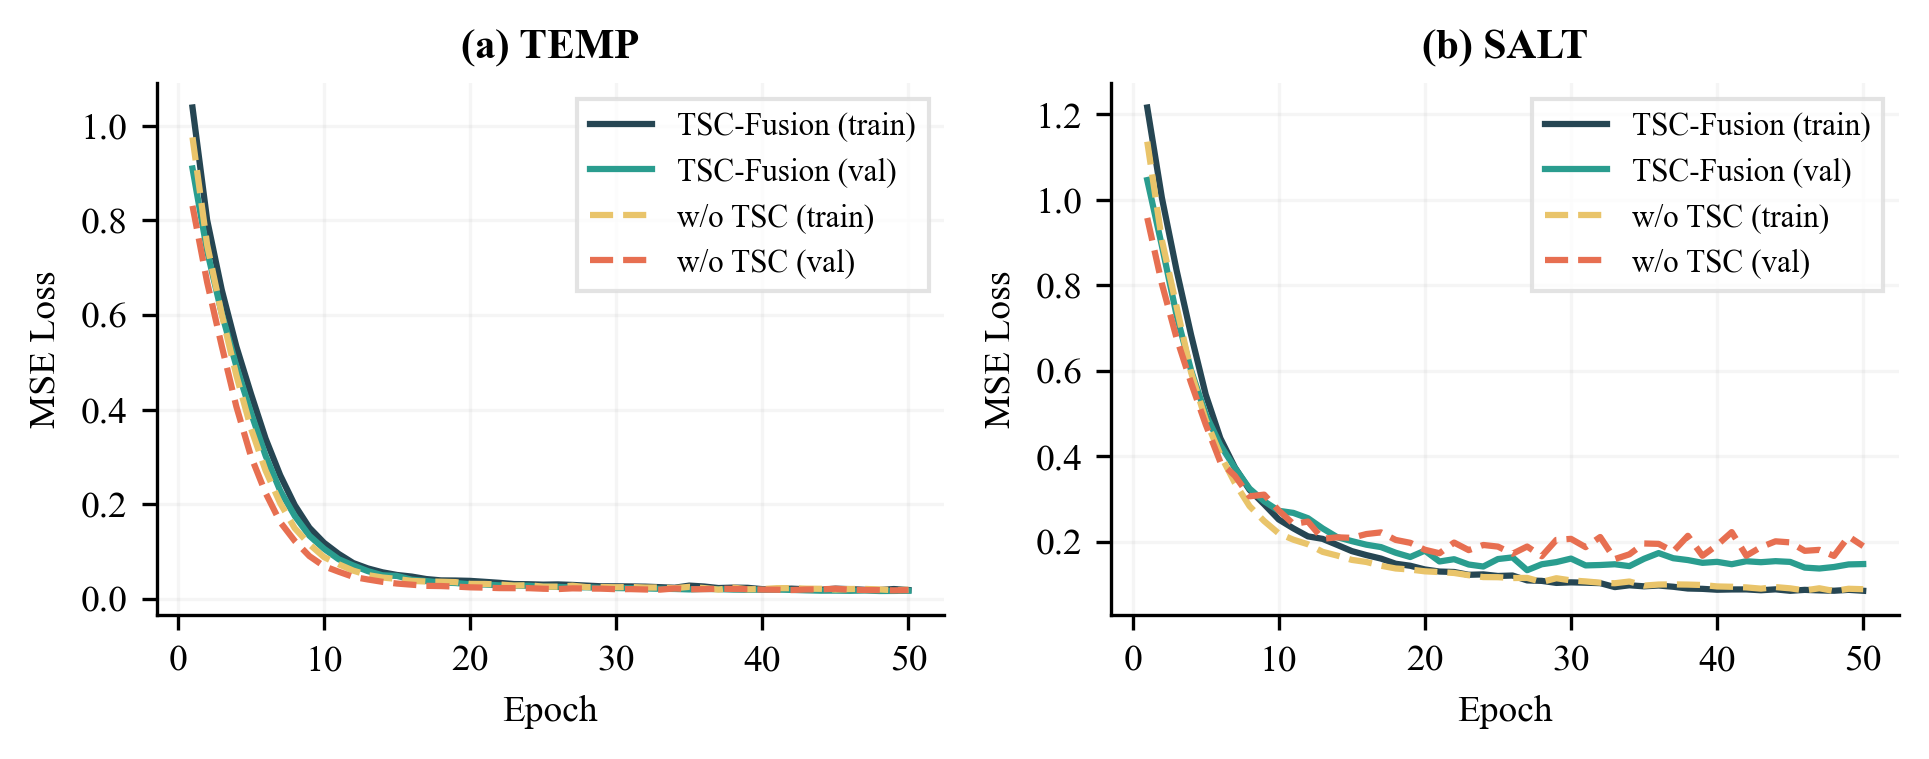
\includegraphics[width=0.94\textwidth]{figures/fig_convergence.pdf}
\caption{Training and validation loss trajectories at 50 epochs for full TSC-Fusion vs.\ w/o TSC memory. (a) TEMP: the TSC-free variant converges faster early but the full model overtakes it around epoch 34. (b) SALT: the full model maintains advantage throughout, with the gap widening after epoch 30.}
\label{fig:convergence}
\end{figure*}

Fig.~\ref{fig:convergence} shows the training and validation loss trajectories for both variables. For temperature (Fig.~\ref{fig:convergence}a), the TSC-free variant converges faster in early epochs: at epoch 10, its validation MSE is 0.0692 compared to 0.1060 for the full model---a 35\% gap. This gap narrows through epoch 20 (0.0246 vs.\ 0.0310), and the two trajectories cross around epoch 34, after which the full model maintains a consistent advantage. At epoch 50, the full model achieves a best validation loss of 0.0168 versus 0.0181 for the TSC-free variant, and on the held-out test set yields RMSE 0.1115 versus 0.1122---a consistent but modest improvement.

For salinity (Fig.~\ref{fig:convergence}b), the convergence pattern differs from temperature. Unlike the pronounced early gap observed for TEMP, the full and TSC-free SALT variants start from nearly identical validation losses at epoch 10 (0.2720 vs.\ 0.2728). This suggests that the TSC water-mass prototypes are immediately informative for salinity---consistent with the fact that salinity distributions are more directly shaped by water-mass mixing and advection processes. The full model maintains a small but consistent advantage through epoch 20 and widens the gap at 50 epochs: the full model achieves best validation loss of 0.1331 versus 0.1591 without TSC, and test RMSE of 0.4901 versus 0.4972. Notably, the TSC-free variant shows minimal improvement from 20 to 50 epochs (test RMSE 0.4968 at 20 epochs vs.\ 0.4972 at 50), while the full model continues to improve (0.4995 vs.\ 0.4901), indicating that the TSC module's water-mass inductive bias not only provides immediate benefit for salinity but also enables more effective use of additional training iterations.

The convergence behavior is consistent with the water-mass prototype hypothesis. The TSC module must first discover meaningful profile clusters from data before the Transformer encoder can propagate useful water-mass context. For temperature, this prototype discovery phase---approximately the first 30--35 epochs---consumes training iterations that, in the 20-epoch regime, would alternatively be used to refine the local convolutional branch. For salinity, the prototypes are directly informative from the start, and extended training primarily refines the prototype-to-context mapping. We recommend a minimum of 30--40 epochs when training TSC-Fusion, particularly for applications where the water-mass inductive bias is expected to provide the largest benefit.

\subsection{Physical Consistency}

Table~\ref{tab:physical} reports TEOS-10-derived physical consistency metrics. The TEOS-10 diagnostics are computed from the denormalized predicted TEMP/SALT fields using the same depth and geographic coordinates as the target data. Because the derived fields (potential density and spiciness) are not directly optimized during training, their prediction quality reflects whether the model has learned physically plausible joint temperature-salinity relationships. TSC-Fusion achieves strong performance on both derived variables, with $R^2$ values of 0.9780 for PDEN and 0.9752 for SPICE---outperforming both baselines---indicating that the TSC memory module and multi-branch fusion preserve meaningful temperature-salinity coupling.

\begin{table}[t]
\centering
\caption{Physical consistency evaluation on TEOS-10 derived variables. RMSE values are reported in the native units of each variable.}
\label{tab:physical}
\footnotesize
\renewcommand{\arraystretch}{1.08}
\begin{tabular}{@{}llccc@{}}
\toprule
\textbf{Metric} & \textbf{Variable} & \textbf{AxiomOcean} & \textbf{FuXi-Ocean} & \textbf{TSC-Fusion} \\
\midrule
\multirow{2}{*}{RMSE}
& PDEN  & 0.3534 & 0.3515 & \textbf{0.3248} \\
& SPICE & 0.3861 & 0.3803 & \textbf{0.3567} \\
\midrule
\multirow{2}{*}{$R^2$}
& PDEN  & 0.9739 & 0.9742 & \textbf{0.9780} \\
& SPICE & 0.9710 & 0.9718 & \textbf{0.9752} \\
\bottomrule
\end{tabular}
\end{table}

\section{Discussion}

The results demonstrate that TSC-Fusion's multi-branch design provides complementary benefits for ocean temperature and salinity prediction. Several observations merit discussion.

First, the TSC memory module introduces an explicit water-mass inductive bias that appears particularly beneficial for salinity. Salinity distributions are strongly shaped by water-mass formation, mixing, and advection; by soft-routing profiles to learned water-mass prototypes and propagating that context through the Transformer encoder, the TSC module captures relationships that are harder for generic convolutional or attention architectures to learn from limited training samples. This interpretation is consistent with the salinity $R^2$ improvement of 2.4 percentage points over the best baseline.

Second, the global spectral branch targets large-scale gradients and basin-scale teleconnections. Ocean temperature, in particular, exhibits strong meridional and zonal gradients driven by solar forcing and large-scale circulation. The Fourier-domain representation enables the model to learn these low-frequency modes with far fewer parameters than would be required by an equivalent spatial-domain convolutional stack.

Third, the 3D spatiotemporal structure branch preserves the joint variable-time-space structure that is lost when variables and time steps are flattened into channels. Ocean vertical structure---the thermocline depth, the salinity maximum, the transition between water masses---depends on interactions across depth, variable, and time dimensions that 2D convolutions cannot directly represent. By operating on the full 4D tensor, the 3D branch captures these interactions explicitly.

Fourth, the gated ensemble head reduces the variance inherent in single-head predictions. Different ensemble members can specialize to different spatial regimes or forecast lead times, and the spatial gate learns to weight them accordingly. This mechanism is analogous to the ensemble spread in numerical weather prediction, but with the weights learned end-to-end from data.

We note two important caveats. First, TSC-Fusion uses additional thermohaline inputs (PTEMP, PDEN, SPICE) that are derived from the same TEMP and SALT fields but encode physically meaningful water-mass properties. The ablation with standard 5-variable input (w/o PTEMP/PDEN/SPICE) isolates how much of the gain comes from the architecture versus the additional input information. Second, the 20-epoch protocol provides a controlled comparison but does not represent the performance ceiling of any model. Longer training, larger hidden dimensions, and learning rate tuning would likely improve all models. The key finding is the strong performance of the complete physically enhanced configuration, together with the component-dependent behavior revealed by controlled ablations.

\section{Conclusion}

We presented TSC-Fusion, a thermohaline-structured fusion network for ocean temperature and salinity prediction that integrates water-mass-aware memory, global spectral low-mode learning, 3D spatiotemporal structure modeling, and gated ensemble fusion. Under a standardized 20-epoch evaluation protocol, TSC-Fusion achieves first-place results on both temperature and salinity against FuXi-Ocean, FuXi-ONS, and AxiomOcean reimplementations. Ablation experiments identify the ensemble gate and thermohaline-derived inputs as the most critical components. The TSC memory shows convergence-dependent benefits under extended training, while the spectral and 3D branches exhibit variable-dependent optimization behavior under the short ablation budget. TEOS-10-derived physical diagnostics further verify that the predicted fields preserve meaningful temperature-salinity coupling. Future work will extend the framework to longer forecast horizons, incorporate additional physical constraints such as the T-S relationship directly into the loss function, and evaluate robustness under extreme ocean-atmosphere events including typhoons and strong ENSO episodes.

\section*{Funding}
This research was supported by Key Laboratory of Southeast Coast Marine Information Intelligent Perception and Application, MNR, No.~24205 and XMU Training Program of Innovation and Entrepreneurship for Undergraduates (S202510384570).

\section*{Acknowledgment}
The authors thank the Global Argo Float Program, AVISO, and CCMP data providers for making the ocean observations available.

\bibliographystyle{IEEEtran}
\bibliography{reference}

\end{document}
